\chapter{Interpolating between hadronic transport and hydrodynamics using forced canonical thermalization}
\label{chap:forced_therm}

This chapter is based on \cite{Oliinychenko:2016vkg}. As discussed in sections
\ref{sec:hydro_appr} and \ref{sec:transport}, the applicability of
hydrodynamics requires that $l_{mfp} \ll L$ and the applicability of transport
requires $l_{mfp} \gg \lambda_{Compton}$, where $l_{mfp}$ denotes mean free
path, $L$ is size of the system and $\lambda_{Compton}$ is typical Compton
wavelength. This complementarity of applicability regions of hydrodynamical and
transport approaches makes hybrid approaches (see section
\ref{sec:hybrid_appr}) theoretically attractive, since in a hybrid approach
each description is assumed to act in its region of applicability. Currently,
the focus in heavy ion collision experiments is shifting towards intermediate
collision energies (see section \ref{sec:HI_exp} for review of heavy ion
experiments), at which the observation of the QCD critical point and the first
order phase transition is expected. At the same time at intermediate energies
the assumptions adopted by hybrid approaches become challenging.

A typical hybrid approach starts with generating an initial state, which can be
highly anisotropic and includes event-by-event fluctuations. Then a rapid
switch to relativistic hydrodynamics is performed, which neglects the initial
anisotropy of the energy-momentum tensor. Hydrodynamical equations are solved
in the forward light-cone until some late time. The particlization hypersurface
(usually a constant temperature, energy density or Knudsen number hypersurface)
is then determined, a Cooper-Frye particlization (section
\ref{sec:cf_explanation}) is performed upon that surface, and particles are
finally allowed to rescatter using hadronic transport. Note that in such
approaches, hydrodynamical equations are solved even out of their region of
applicability, where the Knudsen number is large. The particlization
hypersurface is determined a posteriori from hydrodynamics, but not from a
dynamical condition considering both hydrodynamics and transport. Particles in
the transport phase have no possibility to cause feedback to hydrodynamics,
which leads to a well-known problem, the so-called negative Cooper-Frye
contributions
\cite{Bugaev:1996zq,Bugaev:1999wz,Anderlik:1998cb,Oliinychenko:2014tqa}. At
high collision energies, at midrapidity, which is the kinematical region
studied by RHIC and LHC, negative Cooper-Frye contributions are negligible and
the approximation adopted by hybrid approaches is justified. For lower energies
they were estimated in the chapter \ref{chap:cooper_frye} and can easily reach
the level of 10\% for hydrodynamics with smooth initial conditions. For
event-by-event hydrodynamics they are practically unlimited.

Hydrodynamical and hybrid approaches could be completely substituted by
transport models at low energies, but this presents two challenges. First, the
equation of state does not explicitly enter the transport model, so it becomes
impossible to study the equation of state directly, without specifying the
degrees of freedom. Second, at high densities, multi-particle collisions and
quantum interference effects gain importance, as the applicability condition
$l_{mfp} \gg \lambda_{Compton}$ starts to be violated. As an example, the
account of $p\bar{p}$ annihilations to many mesons and the inverse process of
many-meson collisions is claimed to be essential to describe anti-proton and
anti-Lambda yields at AGS \cite{Cassing:2001ds}, as well as yields at the LHC
\cite{Pan:2014caa}.

Here a simple approach that attempts to solve or avoid the above mentioned
problems is explored. In a pure hadron transport model it is suggested to
perform forced thermalization in the regions of high density. Physically, such
thermalization corresponds to the extreme limit of N-particle collisions, so
intense that thermalization happens rapidly, replacing the local distribution
function by a thermal one. It follows from the H-theorem, that the thermalized
state is unique and independent on the microscopic details of interaction,
which makes it an easy case to consider. In fact such a treatment is
conceptually very similar to a hybrid approach with Smoothed Particle
Hydrodynamics \cite{Aguiar:2000hw}, but here hydrodynamics and transport are
dynamically coupled. Forced thermalization involves the EoS, thus allowing to
explore the phase transition. The method is also similar to core-corona
separation \cite{Steinheimer:2011mp}, but the thermalized and transport domains
are coupled dynamically and transport can feedback to the thermalized regions.
It remains applicable for small systems and at low collision energies, where
hydrodynamics or hybrid approaches are not applicable. All this serves as a
motivation to test and explore the implications of such an approach.

\section{Performing forced canonical thermalization in SMASH}
\label{methodology}

The forced canonical thermalization is implemented on top of the SMASH cascade
approach described in detail in chapter \ref{chap:smash} (specifically the version
SMASH-0.9rc was used). The main assumption of this approach is that if the local rest
frame energy density is high enough rapid thermalization occurs. In practice, the
region $\Omega_{\epsilon_c}$ where the local rest frame energy density $\epsilon$ is
larger than some predefined $\epsilon_c$ is determined and  particles in this region
are substituted by new ones, sampled according to a thermal distribution conserving
total energy, momentum and quantum numbers. In other words, the non-equilibrium
distribution function is replaced by a thermal one in the transport approach at
energy densities $\epsilon > \epsilon_c$. This treatment is ideologically
similar to hybrid (hydrodynamical + transport) approaches, but here the
boundary between the ''hydrodynamical'' and transport regions is found
dynamically and not aposteriori; also negative Cooper-Frye contributions are
not emerging in this approach.

Technically, forced thermalization consists of two steps - coarse-graining to
determine the macroscopic densities and thermodynamic properties and the
sampling of the new particles. To coarse-grain a Cartesian grid is spanned over
the region of interest. The number of cells in each direction is a parameter,
but its variation in a reasonable range does not influence results as shown
later (see section \ref{results}). In each cell, the local energy-momentum
tensor and the four-current are computed according to equations of section
\ref{sec:final_coarse_graining}. In all simulations smearing width $\sigma = 1$ fm is
taken, except for the simulations with the sphere setup, where $\sigma = 0.3$
fm is used to avoid too much smearing and allow for a reasonable comparison of
the results to hydrodynamics. The rest-frame quantities are obtained using Eq.
(\ref{eq:rest_frame_cons}) with an ideal hadron gas equation of state (Eqs.
\ref{eq:id_hadgas_eos1}-\ref{eq:id_hadgas_eos3}).  The list of hadrons in the
equation of state coincides with the list of all hadrons available in SMASH.  This equation of
state is discussed in more detail in section \ref{sec:smash_eos}.

After performing these steps, the information about the local rest-frame energy
density $\epsilon(\vec{r})$, the temperature $T(\vec{r})$, the chemical
potentials $\mu_B(\vec{r})$ and $\mu_S(\vec{r})$, and the local Landau rest
frame velocity $v(\vec{r})$ is available in each cell of the grid. This allows
to construct a region $\Omega_{\epsilon_c}$ where $\epsilon > \epsilon_c$, from
which particles are removed and new ones are sampled according to the local $T$,
$\mu_{B,S}$ and $v$.

Since this sampling procedure is not uniquely defined, let us now discuss a few
possible options. Denote the set of all conserved
quantities (energy, momentum, baryon number, strangeness, electric charge, etc)
in a given event in one cell by $C_{cell}$. The total conserved  quantities in
the thermalization region in this event are $C_{tot} = \sum C_{cell}$, where
the sum goes over all thermalization cells.

The first option is to apply the Cooper-Frye formula to every cell, as it is
done at the particlization in many hydrodynamical models. Then the conservation
laws are fulfilled in every cell, but only in the event average. In the introduced
notations, $\left\langle C_{cell}^{before} \right\rangle = \left\langle
C_{cell}^{after} \right\rangle$, but $C_{cell}^{before} \neq C_{cell}^{after}$.
The framework of a transport approach, used here, strictly
respects conservation laws in each event, therefore it is desirable that the forced
thermalization also follows conservation laws event-by-event.

Another option is to have exact event-by-event conservation laws, where
$C_{tot}^{before} = C_{tot}^{after}$, but $C_{cell}^{before} \neq
C_{cell}^{after}$ and $\left\langle C_{cell}^{before} \right\rangle \neq
\left\langle C_{cell}^{after} \right\rangle$. This approach is applied for
particlization in some hybrid models \cite{Petersen:2008dd, Huovinen:2012is}.
This method is applied here, because it is reasonably fast and provides a very good
approximation to the next approach, when it goes about the distribution of
total (not cell by cell) hadron multiplicities. In the next section the implications
of this choice are investigated and its different algorithmic
implementations are compared. Such a comparison makes this study useful for hybrid
approaches, since it demonstrates how to perform particlization in a faster and more
controlled way.

One more possibility is to perform microcanonical thermalization in each cell,
so that $C_{cell}^{before} = C_{cell}^{after}$. This can in principle be done
using the procedures described in \cite{Werner:1995mx} and
\cite{Becattini:2004rq} for every cell. In this case, it seems that $T$ and
$\mu$ are not necessary, but they are actually useful for initializing the
Metropolis algorithm, as suggested in \cite{Becattini:2004rq}. This method has
two disadvantages: first, Metropolis sampling is slow and the need to perform
it in $\sim 10^4$ of cells makes it almost not feasible. The other disadvantage
is a sensitivity to the cell size and $N_{test}$: indeed, in the case of very
small cells there is typically one or zero particles in the cell. Resampling
this one particle conserving all quantum numbers will most probably lead to no
change at all. At the same time,  increasing $N_{test}$, one will find more
than one particle in such a cell and thermalization results will change. So a
combination of cell size and $N_{test}$ becomes a physical parameter,
characterizing a radius of interaction.

As mentioned, in this calculation the second method is used. The initial
hadrons are substituted by a new set of hadrons distributed with probability

\begin{eqnarray} \label{eq:prob_distr}
  w(\vec{r_i},p_{i}) \sim \prod_{\mathrm{sorts}}\frac{1}{N_{sort}!}
   \prod_{i=1}^N \frac{d^3 \vec{r_i} d^3\vec{p_i}}{(2\pi\hbar c)^3}
   e^{-(p^{\nu}_i u_{\nu}(\vec{r_i}) + \mu_i(\vec{r_i}))/T(\vec{r_i})}
   \delta_E \delta_{\vec{p}} \delta_B \delta_S \delta_C \,,
\end{eqnarray}

where $N_{sort} denotes the multiplicity of a hadron specie.
$The $\delta$-functions in this expression denote the conservation of total
energy, momentum, baryon number, strangeness and electric charge. All these
quantum numbers should be equal to the quantum numbers of initial particles in
the region $\Omega_{\epsilon_c}$. Without the $\delta$-functions, the sampling
distribution from Eq. \ref{eq:prob_distr} is equivalent to a Cooper-Frye
sampling on an isochronous hypersurface. In this case by integrating over $d^3
\vec{r_i} d^3\vec{p_i}$ one can easily see that the distribution of a
particular hadron yield in one cell is Poissonian:

\begin{eqnarray}
\label{eq:pois}
  w(N_{i}) \sim \frac{(V_{cell}\varphi_i)^{N_i}}{N_i!} \\
  \varphi_i = \frac{g_i e^{\mu/T}}{(2\pi\hbar c)^3}\int d^3p \, e^{-p^{\nu} u_{\nu}/T}
\end{eqnarray}

where $\varphi_i$ is the average equilibrium density of a given hadron species
in the cell. Strictly speaking, in a case with total energy- and momentum
conservation this consideration is not applicable any more, because now
momentum integrations involve additional global $\delta$-functions, so the
distribution in one cell may be different from Poissonian. However, it is assumed
that there are many cells with many particles in them, so that the global
conservation laws affect the local Poisson distributions only slightly. From
these considerations it is clear, that the method prefers larger $N_{test}$ and
not too large cells to achieve reliable results. The details of the sampling
algorithm and a test in a thermal box are discussed in the next section
\ref{box_test}.

Here Boltzmann statistics was assumed instead of more realistic Fermi-Dirac and
Bose-Einstein statistics. This is done intentionally to be consistent with the
absence of Pauli-blocking or Bose-enhancement effects in the transport
simulation. For quantum statistics the multiplicity distribution in a cell is
not Poissonian anymore. For bosons the mean multiplicity increases due to
quantum statistics and the variance decreases, for fermions it is the opposite.
Here our model is applied for low collision energies in the high-density region, where
the typical temperatures are around 110 MeV and typical baryon chemical
potentials are of order 700 MeV (see Fig. \ref{Fig:AuAu_Tmu}). The correction
for pions is then $\frac{1}{2} \frac{K_2(2m_{\pi}/T)}{K_2(m_{\pi}/T)} \approx 7
\%$, for protons it is $\frac{1}{2} \frac{K_2(2m_p/T)}{K_2(m_p/T)} e^{\mu/T}
\approx 4 \%$ and for all the other hadrons it has to be smaller.

The forced thermalization is performed every $\Delta t_{th}$ starting from time
$t_{start}$. Unless stated otherwise, $t_{start} = 0$ fm/c and $\Delta
t_{th} = 1$ fm/c are taken. Further $\Delta t_{th}$ is varied to see its effect on
observables in Section \ref{results}. The system evolution before, between and
after thermalizations follows the conventional SMASH cascade, with propagation,
collisions and decays. It is assumed that the N-particle collisions happen
momentarily, at a single point in time.

\section{Thermal box - testing the sampling algorithm}
\label{box_test}

\begin{figure}
  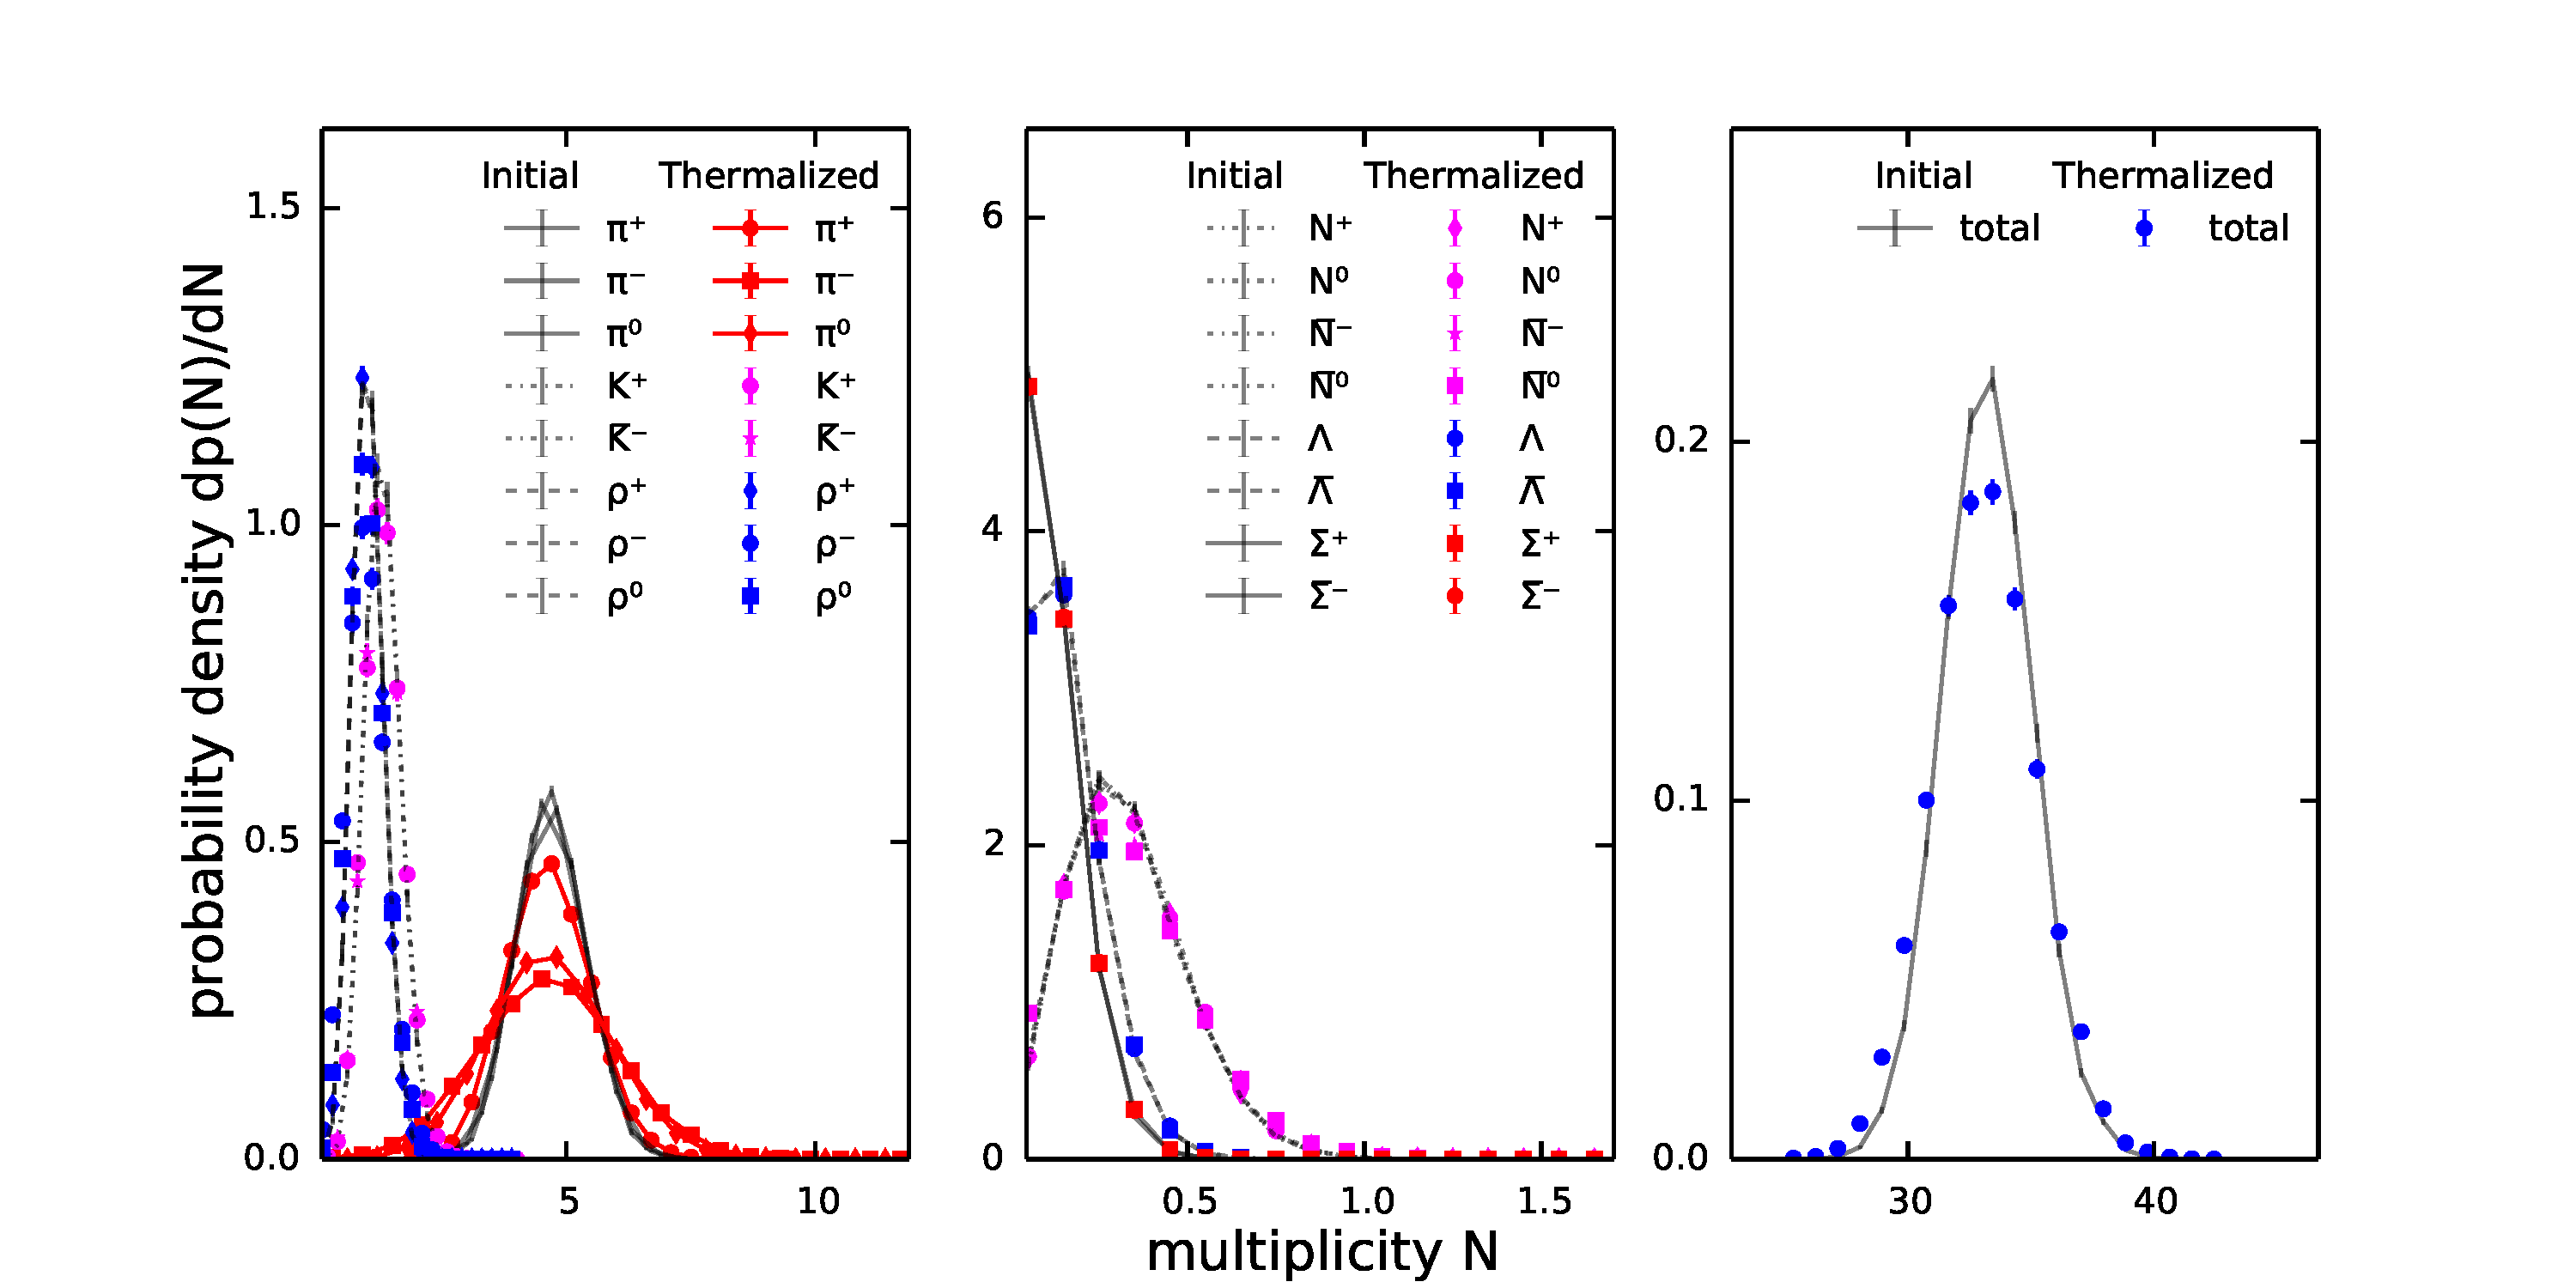
\includegraphics[width=\textwidth]{plots/forced_thermalization/modes_sampling.pdf}
  \caption{Multiplicity distributions in a thermally initialized box are
           compared before and after additional forced thermalization. For a perfect
           thermalization algorithm these distributions should coincide. Here the
           thermalization algorithm is mode sampling.}
  \label{Fig:modes_sampling}
\end{figure}

Thermalization with global conservation of quantum numbers can be performed
with different algorithms. In this section, three algorithms are compared within
a thermal box containing infinite hadronic matter in equilibrium. First,
a $V = (5$ fm$)^3$ box with periodic boundary conditions is created and initialized
with thermally distributed hadrons that are available in SMASH. The multiplicities
of each hadron species are $N_i = Poi(\phi_i)$, where $Poi$ is a Poisson
distribution and $\phi_i$ is the thermal multiplicity of $i$-th hadron species
at a temperature of $T = 0.15$ GeV and zero chemical potential $\mu_B = 0$. The
values of temperature and chemical potential are an arbitrary choice, but they
correspond to the relevant conditions in hybrid approaches for heavy ion
reactions at high beam energies. The initial momenta are sampled from the
Boltzmann distribution with the same temperature. The momenta in the box are
centralized, so that total momentum of the box is zero, $p_i := p_i -
\frac{1}{N}\sum_{j=1}^N p_j$. In this way a box with a thermalized
hadron gas is obtained. The total energy and quantum numbers of such a box fluctuate
from event to event.

As a second step the thermalization algorithm is applied, which conserves total
energy, momentum and quantum numbers as described above in Section
\ref{methodology}. The space-time grid consists of $10^3$ cells. On this grid,
the coarse graining as described above is performed, taking the periodic
boundary conditions into account. After sampling new particles with three
different algorithms the initial multiplicity and momentum distributions with
the ones after forced thermalization are compared. If everything works as
expected, the results are supposed to be identical.

The first algorithm under investigation is the mode sampling used for
particlization in the UrQMD hybrid approach \cite{Huovinen:2012is}. It consists
of seven steps called ''modes'':
\begin{enumerate}
  \item Choose a cell with probability $\frac{V_{cell}}{V}$. Sample particles
        in the cell according to the thermal distribution assuming a Poisson
        distribution around the mean, until the total energy exceeds $E_{init}$. Only
        particles with the positive strangeness are kept, reject all the other
        particles.
  \item Compensate strangeness by sampling only particles with the negative strangeness.
  \item Sample non-strange hadrons until the total energy exceeds $E_{init}$,
        keeping only non-strange baryons.
  \item Compensate baryon charge by sampling only anti-baryons.
  \item Sample non-strange mesons until the total energy exceeds $E_{init}$,
        keeping only positively charged non-strange mesons.
  \item Compensate electric charge by sampling negatively-charged non-strange mesons.
  \item Sample neutral mesons until the energy is conserved.
\end{enumerate}

In this work, the original mode sampling algorithm has been improved to
increase the computational speed. Choosing the cell with the  probability
$\frac{N_{cell}}{\sum_{cells} N_{cell}}$ and sampling one particle definitely
in there helps to avoid rejections and samples the same distribution in a
faster way. This improvement is especially noticeable at high baryon chemical
potential, such as the one reached in low energy heavy ion collisions. The
average total number of anti-baryons can then be order of $10^{-5}$. Sometimes
one or two anti-baryons are needed to compensate the baryon number, but the
probability to sample one in the original algorithm is $10^{-5}$ divided by
number of cells. Therefore, many rejection steps are avoided with the newly
defined probability.

Applying the mode sampling within the thermal box (see Fig.
\ref{Fig:modes_sampling}), one observes that the mean values of multiplicities
are all reproduced and many multiplicity distributions are also reproduced.
However, the $\pi$ and $\rho$ multiplicity distributions are wider than the
initial ones, which results in a wider distribution for the total multiplicity.
Moreover, the width of the multiplicity distribution follows $\Gamma(\pi^-) >
\Gamma(\pi^0) > \Gamma(\pi^+)$, and similarly for $\rho$-mesons. To find the
origin of this deviation from the expectation, the mode sampling order has been
exchanged - instead of keeping only positively charged first and compensating
with negative particles, only negatively charged are kept first and compensated
with positive afterwards. Such reverse procedure results in $\Gamma(\pi^+) >
\Gamma(\pi^0) > \Gamma(\pi^-)$. This demonstrates that the multiplicity distribution
obtained from the mode sampling is sensitive to the internal algorithm realization,
which is not physical.

\begin{figure}
  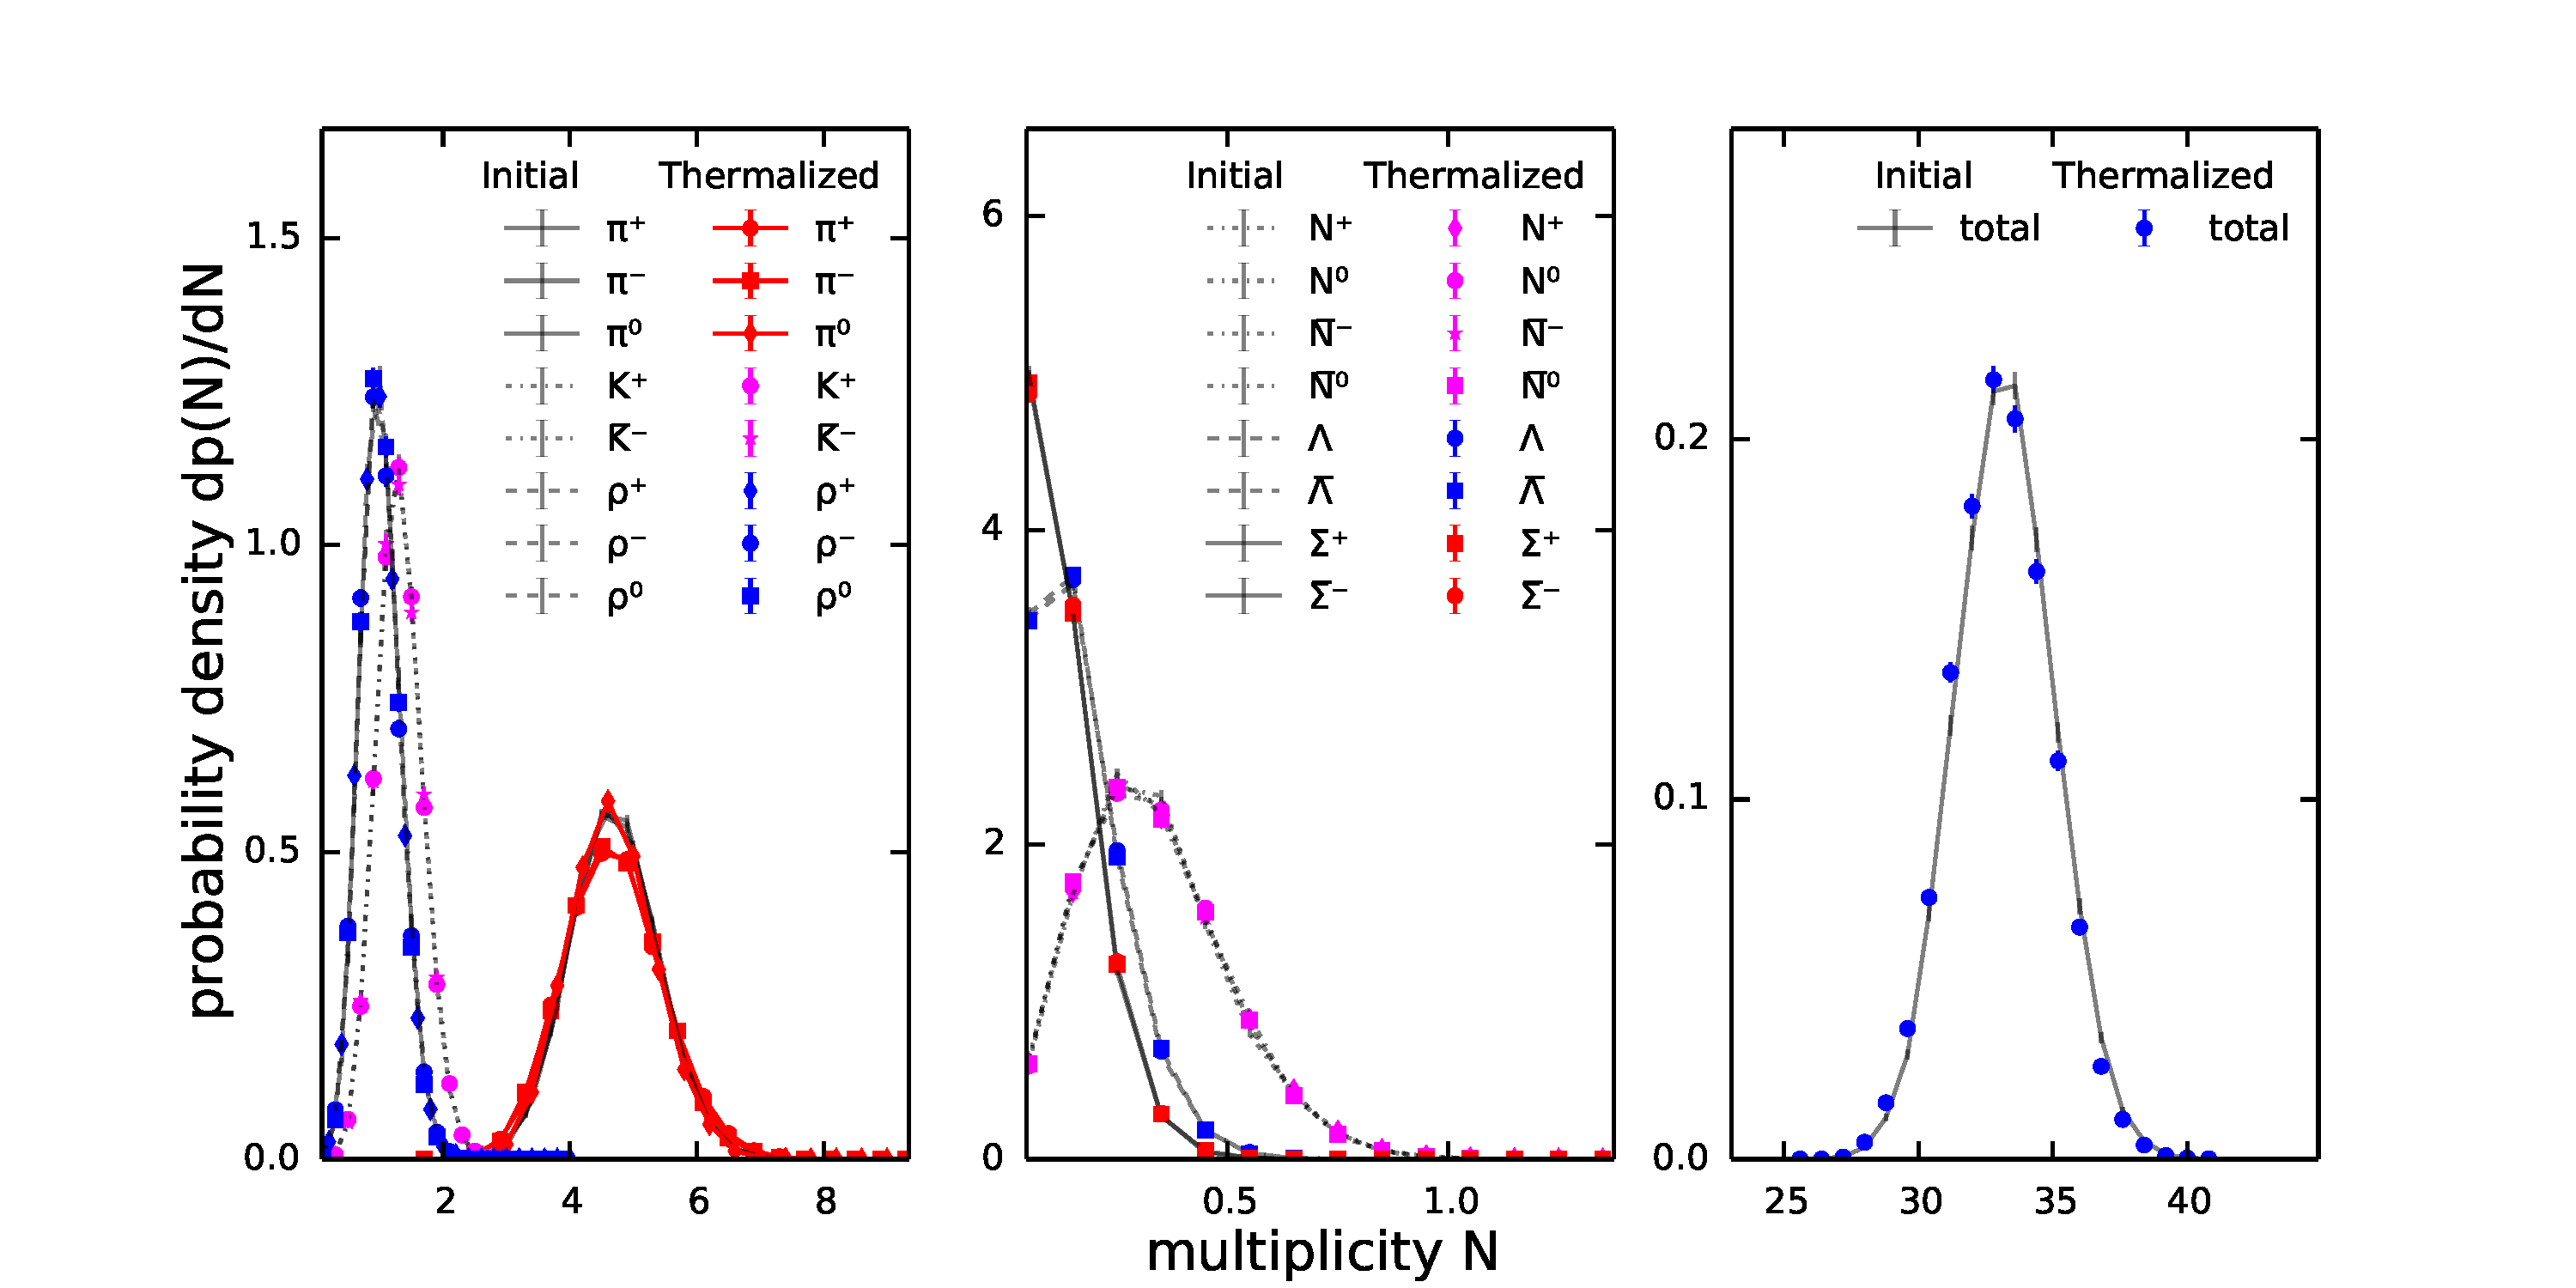
\includegraphics[width=\textwidth]{plots/forced_thermalization/BF_biased.pdf}
  \caption{Multiplicity distributions in a thermally initialized box are
           compared before and after additional forced thermalization. For a perfect
           thermalization algorithm these distributions should coincide. Here the
           thermalization algorithm is biased Becattini-Ferroni sampling with rejection by
           total energy.}
  \label{Fig:biasedBF_sampling}
\end{figure}

The second considered algorithm is following the idea suggested by Becattini
and Ferroni in \cite{Becattini:2004rq}, where one takes advantage of the fact
that the sum of Poissonian variables is Poissonian itself. However, we
implemented a biased version, different from the original Becattini and Ferroni
suggestion. This version turns out to be numerically more efficient, while the
bias is rather modest. The algorithm consists of the following steps:

\begin{enumerate}
  \item Compute total average thermal numbers of baryons $\nu_{B}$ and
        anti-baryons $\nu_{\bar{B}}$. Sample $N_B$ and $N_{\bar{B}}$ with probability

    \begin{equation}
      w(N_B, N_{\bar{B}}) \sim \frac{\nu_{B}^{N_B}}{N_B!}
      \frac{\nu_{\bar{B}}^{N_{\bar{B}}}}{N_{\bar{B}}!} \delta(N_B - N_{\bar{B}} = B_{init}) \,.
    \end{equation}

        Such a distribution can be sampled very efficiently using the method discussed
        in the Appendix. Then the multiplicities of particular baryons and anti-baryons
        are sampled from the multinomial distribution.
  \item Compute total thermal average  for strange and anti-strange mesons:
        $\nu_{S}$ and $\nu_{\bar{S}}$. Then sample $N_S$ and $N_{\bar{S}}$ with distribution

    \begin{equation}
      w(N_S, N_{\bar{S}}) \sim \frac{\nu_{S}^{N_S}}{N_S!}
      \frac{\nu_{\bar{S}}^{N_{\bar{S}}}}{N_{\bar{S}}!}
      \delta(N_S - N_{\bar{S}} = S_{init} - S_{\mathrm{sampled}}) \,.
    \end{equation}

        Then particular numbers of strange and anti-strange mesons are sampled from
        multinomial distribution.
  \item Same procedure for charged non-strange mesons, in the distribution
        there is $\delta(N_C - N_{\bar{C}} = C_{init} - C_{\mathrm{sampled}})$, where
        $C_{\mathrm{sampled}}$ is the charge of the hadrons sampled in the previous
        steps.
  \item Sample numbers of neutral mesons from Poissonian distributions.
\end{enumerate}

Notice that for this version of the algorithm the distribution of the total
number of particles is too wide. It turns out that this effect can be
decreased, if one rejects all samples where the energy is too far away from the
initial energy. Rejecting $|E_{sampled} - E_{init}|/E_{init} > 1\%$, one obtains
the correct distribution for the total multiplicity, but the sampled
distributions for $\pi$ and $\rho$ are slightly wider than the initial ones,
see Fig. \ref{Fig:biasedBF_sampling}. This algorithm is so efficient, because
of the fast method to generate pairs of Poisson-distributed numbers with fixed
difference, described in the Appendix. The simple rejection method used for
this purpose in the original paper by Beccatini and Ferroni is fast enough for
the case of small chemical potential, but becomes slow for $\mu_B \simeq 0.7$
GeV reached in the Au+Au collisions at $\sqrt{s} = 3$ GeV - the energy relevant
for our investigation.

\begin{figure}
  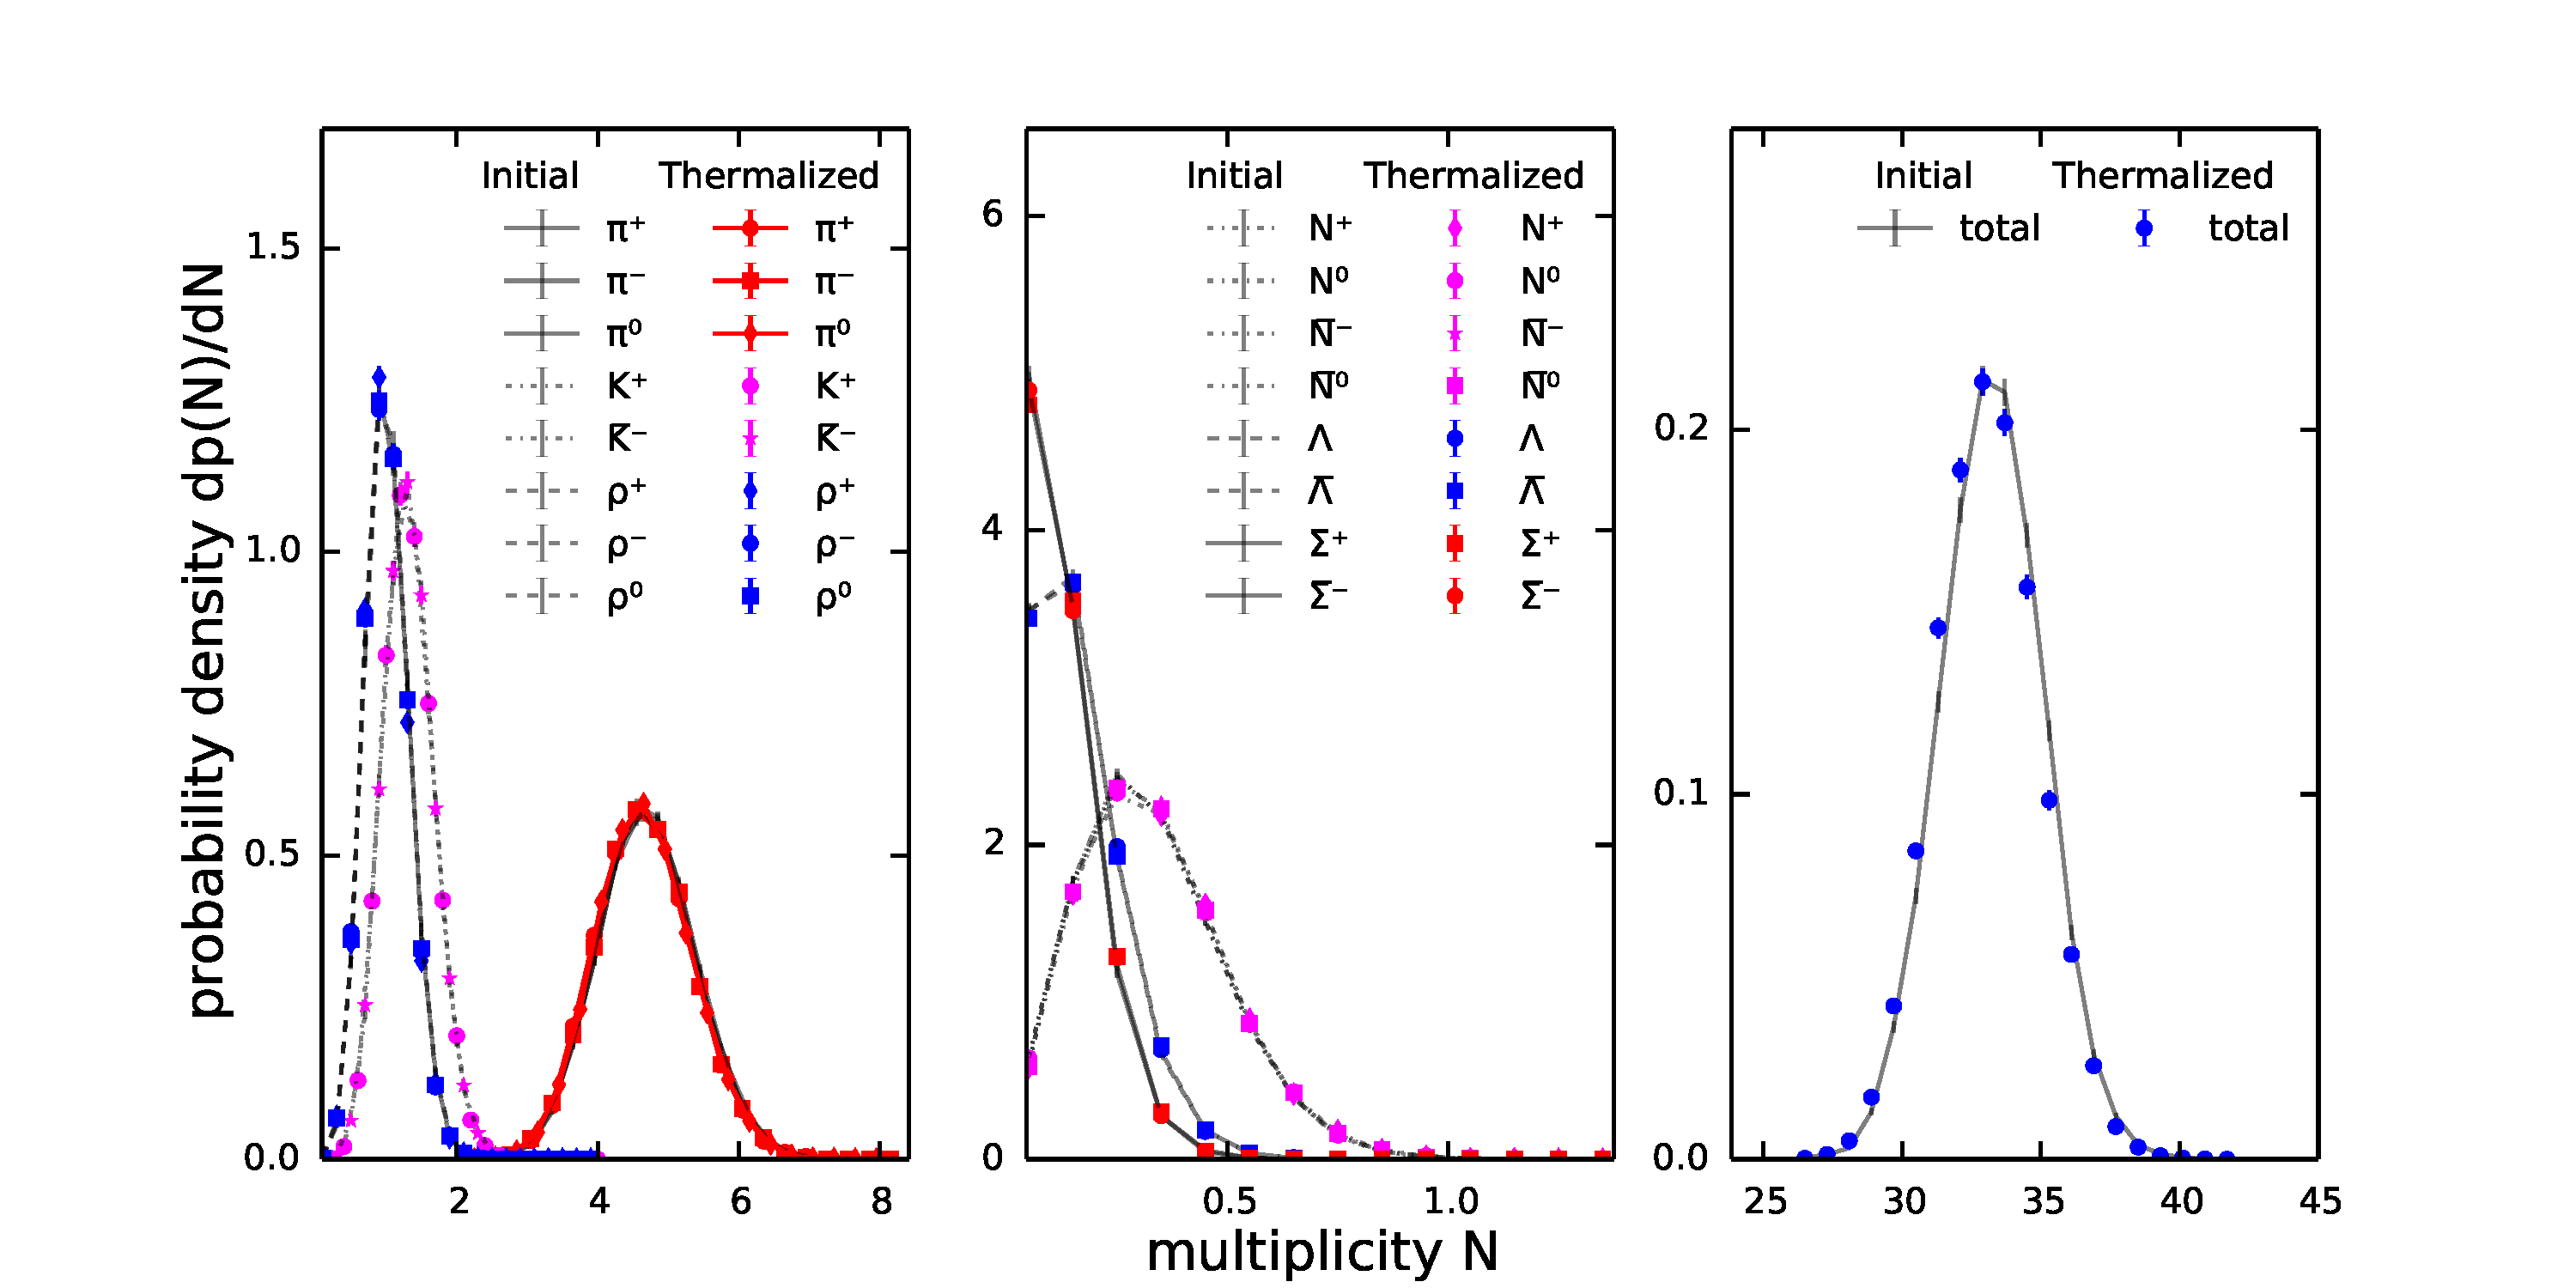
\includegraphics[width=\textwidth]{plots/forced_thermalization/BF_unbiased.pdf}
  \caption{Multiplicity distributions in a thermally initialized box are
           compared before and after additional forced thermalization. For a perfect
           thermalization algorithm these distributions should coincide. Here the
           thermalization algorithm is the unbiased Becattini-Ferroni sampling with
           rejection by total energy.}
  \label{Fig:BFefix_sampling}
\end{figure}

Finally, the unbiased algorithm is tested, which is very similar to the previous one,
 except that rejection at any step requires the algorithm to start from scratch.

\begin{enumerate}
  \item Identical to the first step of the biased algorithm.
  \item Compute total thermal average for strange and anti-strange mesons:
        $\nu_{S}$ and $\nu_{\bar{S}}$. Then sample $N_S = Poi(\nu_{S})$
        and $N_{\bar{S}} = Poi(\nu_{\bar{S}})$. If $N_S - N_{\bar{S}} = S_{init} -
        S_{\mathrm{sampled}}$, then proceed further, else start from the very
        beginning.
  \item Similar to previous step for electric charge. If charge conservation not
        fulfilled, start over from the first step.
  \item Sample neutral non-strange mesons.
  \item Sample momenta for all particles, if total energy deviates more than 1\% from
        the initial energy start over from the first step.
\end{enumerate}

This algorithm produces the correct multiplicity distributions (see Fig.
\ref{Fig:BFefix_sampling}). Finally, Fig. \ref{Fig:BFefix_sampling_energy}
shows that the energy distributions are also appropriate using this algorithm.

\begin{figure}
  \centering
  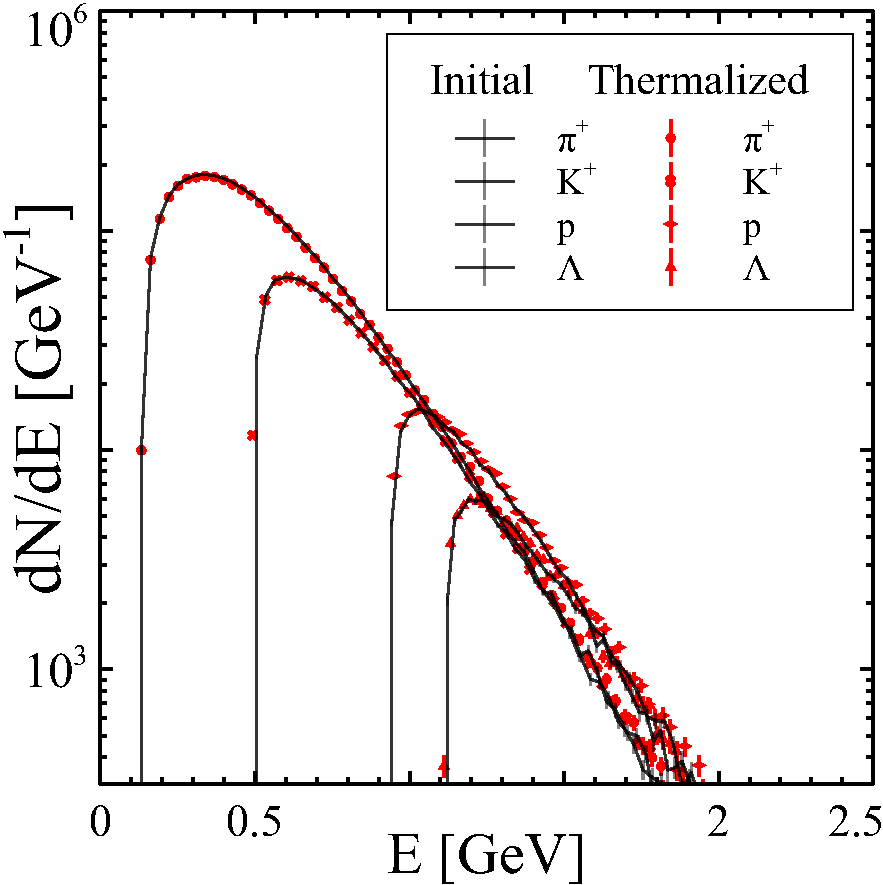
\includegraphics[width=0.5\textwidth]{plots/forced_thermalization/E_spectra_box_test.pdf}
  \caption{Thermal box with the unbiased Becattini-Ferroni sampling with
           rejection by total energy: testing energy distribution}
  \label{Fig:BFefix_sampling_energy}
\end{figure}

In the following, the biased Becattini-Ferroni sampling is employed, since it
is more efficient, the bias is small and it does not suffer from internal
dependencies like the mode sampling. For a few cases, it was also checked that the
unbiased algorithm produces identical results. In Fig. \ref{Fig:algo_compar} we
compare the performance of the considered algorithms on an Intel(R) Xeon(R) 2.5
GHz CPU. For the summary of algorithm properties see Tab.
\ref{Tab:algo_summary}.

\begin{figure}
  \centering
  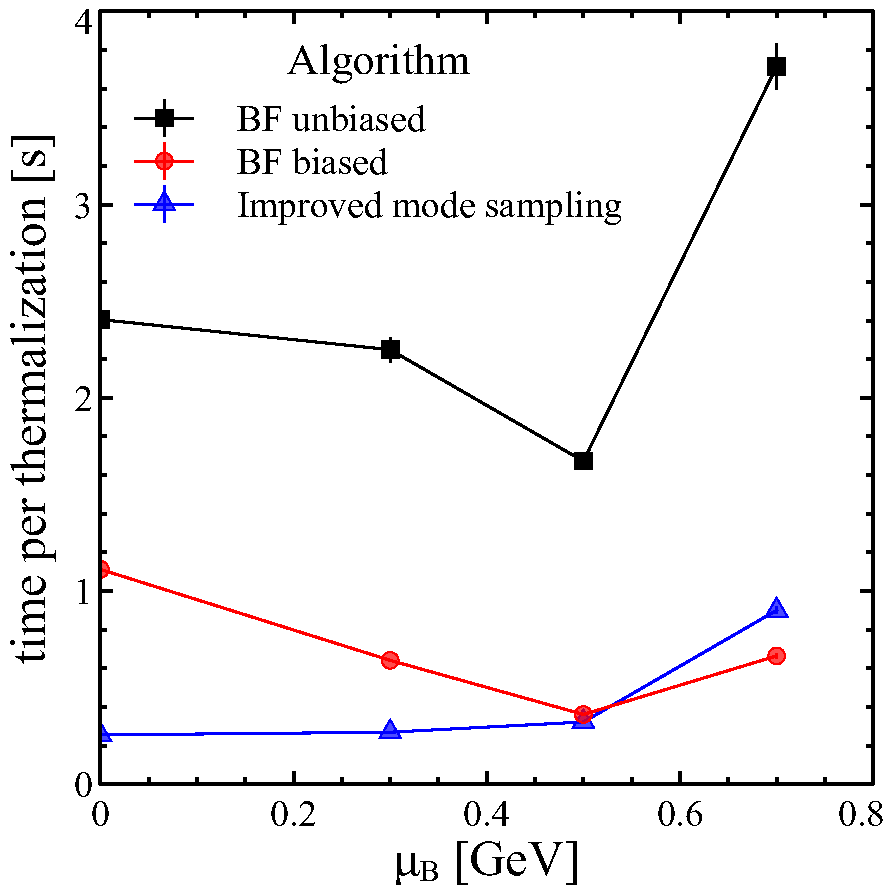
\includegraphics[width=0.5\textwidth]{plots/forced_thermalization/algo_runtime.pdf}
  \caption{Performance comparison of sampling algorithms: mode sampling, biased
           and unbiased Becattini-Ferroni sampling. Thermalization of the $(5$ fm$)^3$
           thermal box with $T = 0.15$ MeV, $N_{test} = 10$, $\mu_S = 0$, $\mu_B$ is
           varied.}
  \label{Fig:algo_compar}
\end{figure}

After the application of the sampling algorithm quantum numbers are conserved,
but energy is only conserved with 1\% precision and momentum conservation is
only fulfilled on average. This shortcoming is addressed in two steps. First,
the momenta are corrected to match the initial momentum, $p_i := p_i -
\frac{1}{N}(\sum_{j=1}^N p_j - p_{init})$. Then, the particles are boosted to the rest
frame of initialization with 3-velocity $-\frac{p_{init}}{E_{init}}$. In this
frame the sum of momenta is zero, because in the previous step
$\sum_{j=1}^N p_j = p_{init}$ was forced, so if one scales all momenta with the same
factor, the sum will remain zero. Therefore, all momenta are scaled with a factor
$(1+a)$, such that

\begin{equation}
  \sum_{j=1}^N \sqrt{m_j^2 + (1+a)^2 p_j^2} = E'_{init}
\end{equation}

Finally the particles are boosted back to computational frame and now energy and
momentum are exactly conserved. This procedure biases momentum distributions,
but this bias decreases with higher numbers of sampled particles $N$. One can
observe in Fig. \ref{Fig:BFefix_sampling_energy}, that if $N$ is large enough,
this bias is negligible.

\begin{table}
\caption{Sampling algorithms with total quantum numbers conservation}
\footnotesize
\begin{tabular*}{\textwidth}{@{}l*{15}{@{\extracolsep{0pt plus12pt}}l}}
\toprule[1.5pt]
Name & Bias on multiplicity distributions & Performance \\
\midrule[1pt]
Mode Sampling & \begin{tabular}{@{}l@{}} Widths of distributions affected,\\ bias dependent on implementation \end{tabular} & fast\\
Biased Becattini-Ferroni & \begin{tabular}{@{}l@{}}  Widths of distributions affected,\\ small bias observed \end{tabular} & comparable to Mode Sampling \\
Unbiased Becattini-Ferroni & No bias observed & $\simeq 4$ times slower than previous\\
\bottomrule[1.5pt]
\end{tabular*}
\label{Tab:algo_summary}
\end{table}


\section{Interpolating between transport and hydrodynamics}
\label{results}

\begin{figure}
  \centering
  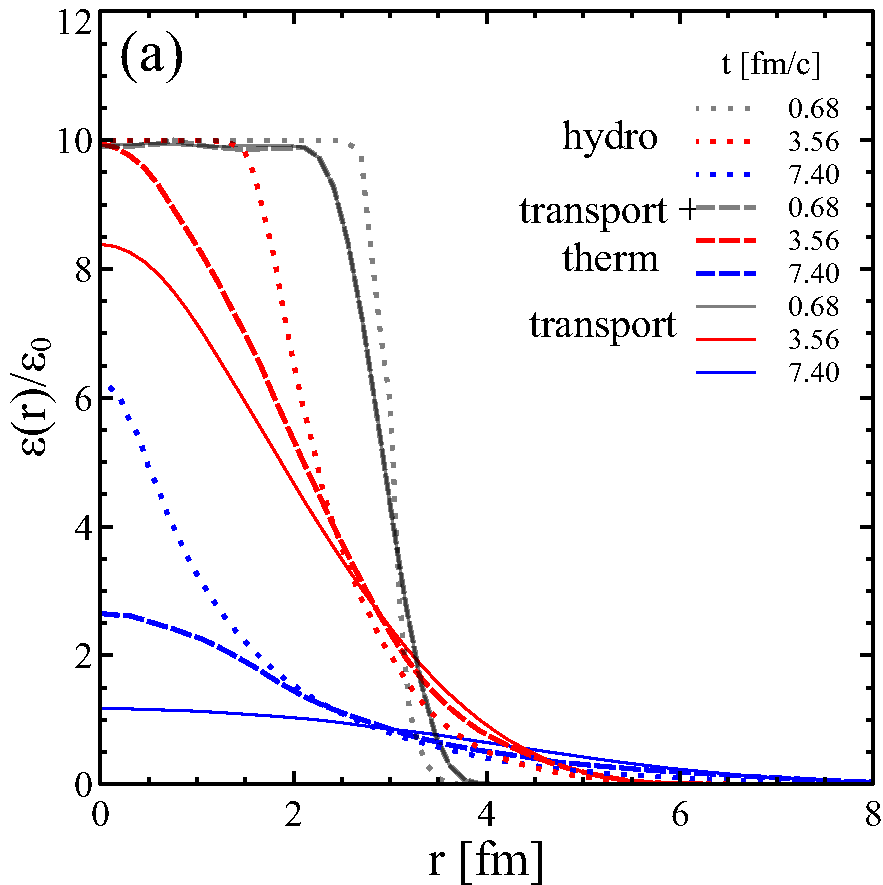
\includegraphics[width=0.49\textwidth]{plots/forced_thermalization/sphere_e_lin.pdf}
  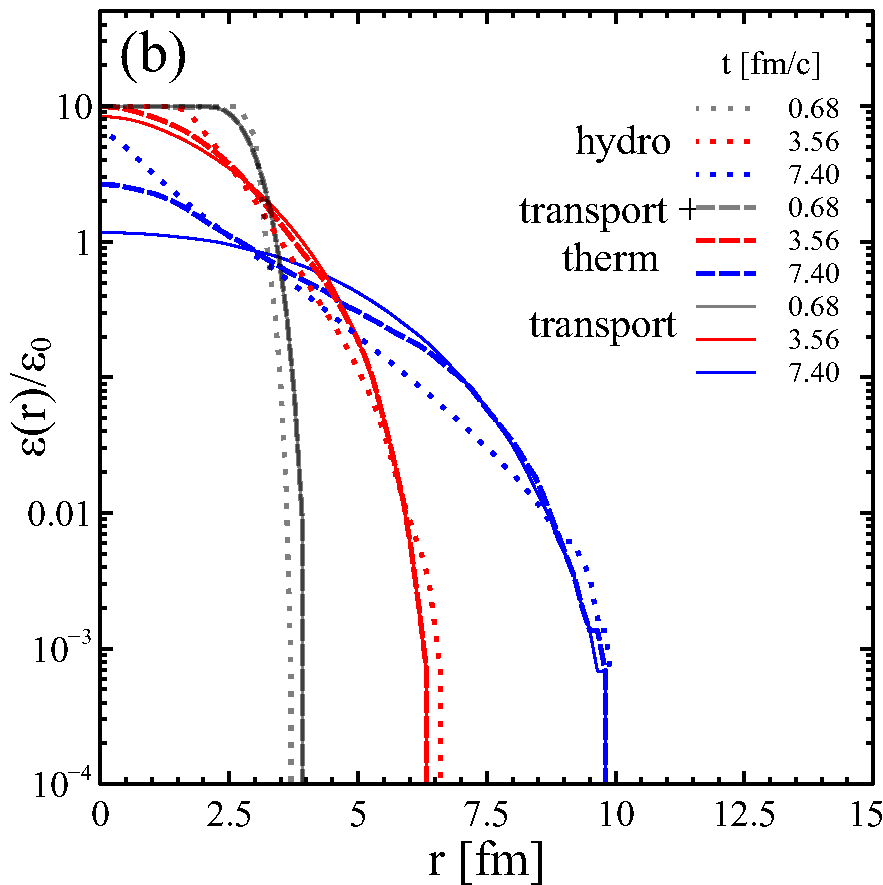
\includegraphics[width=0.49\textwidth]{plots/forced_thermalization/sphere_e_log.pdf} \\
  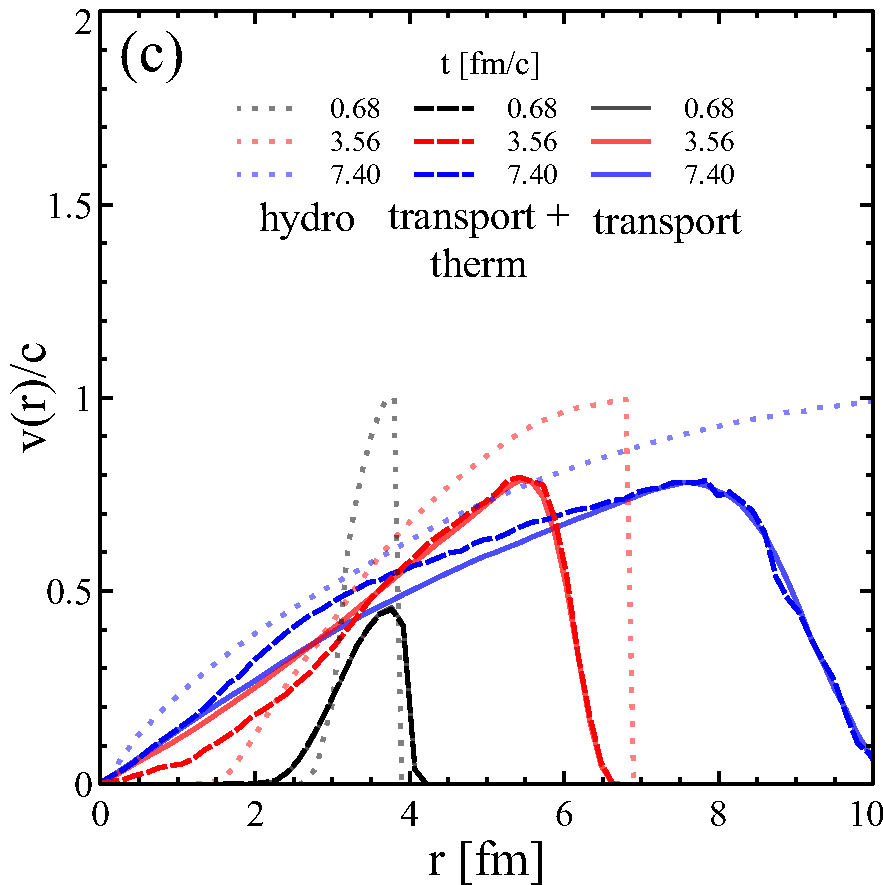
\includegraphics[width=0.49\textwidth]{plots/forced_thermalization/sphere_v.pdf}
  \caption{The time evolution of an expanding sphere is compared for ideal
           hydrodynamics (SHASTA, dotted lines), hadron cascade (SMASH, solid lines)
           and
           the same hadron cascade enhanced by effective N-particle collisions using
           forced thermalization (SMASH+therm, dashed lines). Panels (a) and (b) depict
           the energy density in the local Landau rest frame versus radius. Panel (b)
           is
           exactly the same plot as panel (a) with a logarithmic scale, which allows to
           see the edges of the system. Panel (c) demonstrates the velocity of the
           Landau
           rest frame versus radius. }
    \label{Fig:sphere}
\end{figure}


After establishing the details of the algorithm to effectively include
N-particle collisions in a transport approach, let us compare the influence on the
time evolution of an expanding system to pure transport and ideal fluid
dynamics. The objective is to prove that this dynamically
coupled approach interpolates between the two limits of kinetic theory. For
this purpose, a simple scenario is chosen, namely an expanding sphere. The
sphere of radius $R_0 = 3$ fm is initialized at an energy density of 10 times
nuclear ground state energy densities, $\epsilon = 10\epsilon_0$, and at zero
baryon density. In Fig. \ref{Fig:sphere} the evolution of the local Landau rest
frame energy density and velocity as a function of the radius $r$ are compared.
The ideal hydrodynamics code has been performed using the SHASTA
\cite{Rischke:1995ir} ideal fluid dynamics solver, which uses a $200^3$
Cartesian grid with $0.1$ fm grid spacing in each direction. The time step in
SHASTA is 0.04 fm/c. In SMASH, the sphere is initialized with a thermal hadron
gas with a temperature of $T \approx 191$ MeV, corresponding to energy density
$\epsilon = 10\epsilon_0$. To minimize the effects of smoothing, the
width of the Gaussian smearing kernel is taken to be $\sigma = 0.3$ fm. This is
compensated by taking $N_{test}$ = 100. In the version of SMASH with the effect of
N-particle collisions, forced thermalization is performed every $\Delta t_{th} = 1$
fm/c in the region, where energy density is above $2\epsilon_0$. The thermalization
grid has a cell spacing of 0.5 fm, which can seem rather large, but it was
checked that decreasing it by factors of 2 and 3 does not change the results. 

In Fig. \ref{Fig:sphere} one immediately notices that transport and fluid
dynamics do not produce identical results, as expected. At the time when, in
fluid dynamics, the rarefaction wave has still not reached the center, in
transport the energy density at the center has already dropped. To understand
this difference, one has to consider the Knudsen number in the transport case.
At small times, the scattering rate in SMASH is 0.73 fm$^{-1}$, so that the
mean free path is $l_{mfp} \simeq 1.5$ fm and $Kn \simeq \frac{l_{mfp}}{R_0}
\simeq 0.5$. At this Knudsen number hydrodynamics is already on the verge of
applicability. Moreover, this number is averaged over space and over various
hadron species. On the edges of the system one has to compare the mean free
path not to $R_0$, but to the distance to the edge. Furthermore, some hadron
species have small interaction cross-sections with other particles, so their
mean free path is large and they are in the ballistic regime, not in the
hydrodynamic one. In Fig. \ref{Fig:sphere}, panel (c) shows that velocity at
the edge in the hydrodynamics is $c$, while it is smaller in the transport
model, because of massive particles being present.

SMASH including the effective treatment of N-particle collisions exhibits
intermediate behaviour between hydrodynamics and pure transport. At the edges
of the system, where forced thermalization is not happening, it behaves like
transport, while in the center, it is closer to hydrodynamics. By forcing
thermalization every $\Delta t_{th} = 1$ fm/c, the Knudsen number at the center
is fixed for some time to $Kn \simeq \frac{\langle v_{therm} \rangle \Delta
t_{th} }{R_0}$ for all hadron species. So even for hadrons with small
cross-sections it becomes hard to escape the center too early. In fact, one can
regulate this closeness to hydrodynamics by changing $\Delta t_{th}$. For
smaller $\Delta t_{th}$ one obtains smaller Knudsen number and the result is
thus closer to hydrodynamics. It has to be underlined that the region of forced
thermalization is coupled to the outside region: particles can move in both
directions. This is different from hybrid approaches, where particles from
transport have no chance to feedback to hydrodynamics. Overall, the
introduction of effective N-particle collisions has the expected effect that it
interpolates between pure transport and ideal hydrodynamics. 

% in heavy ion collisions
\begin{figure}
  \centering
  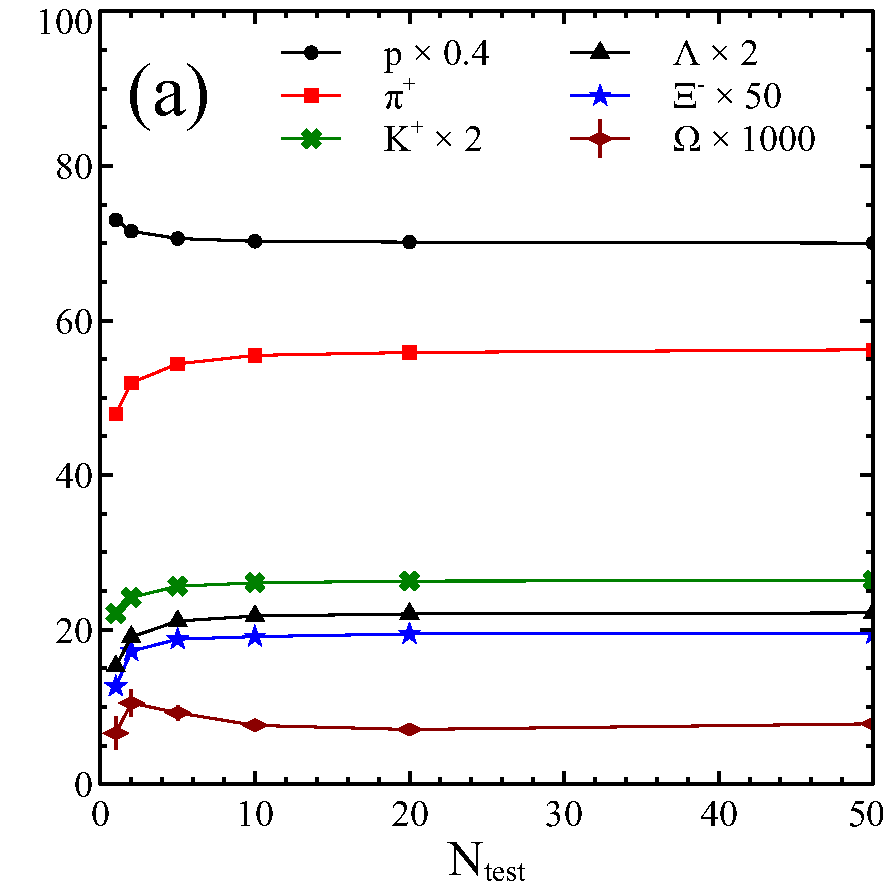
\includegraphics[width=0.49\textwidth]{plots/forced_thermalization/mult_ntest.pdf}
  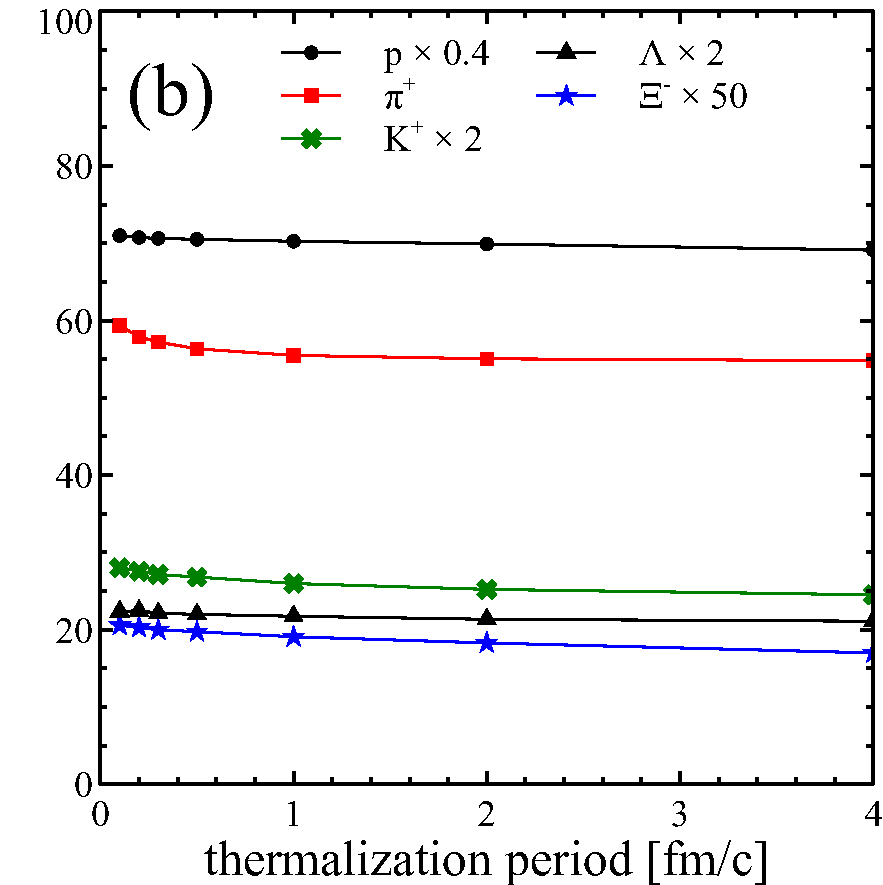
\includegraphics[width=0.49\textwidth]{plots/forced_thermalization/mult_dt.pdf} \\
  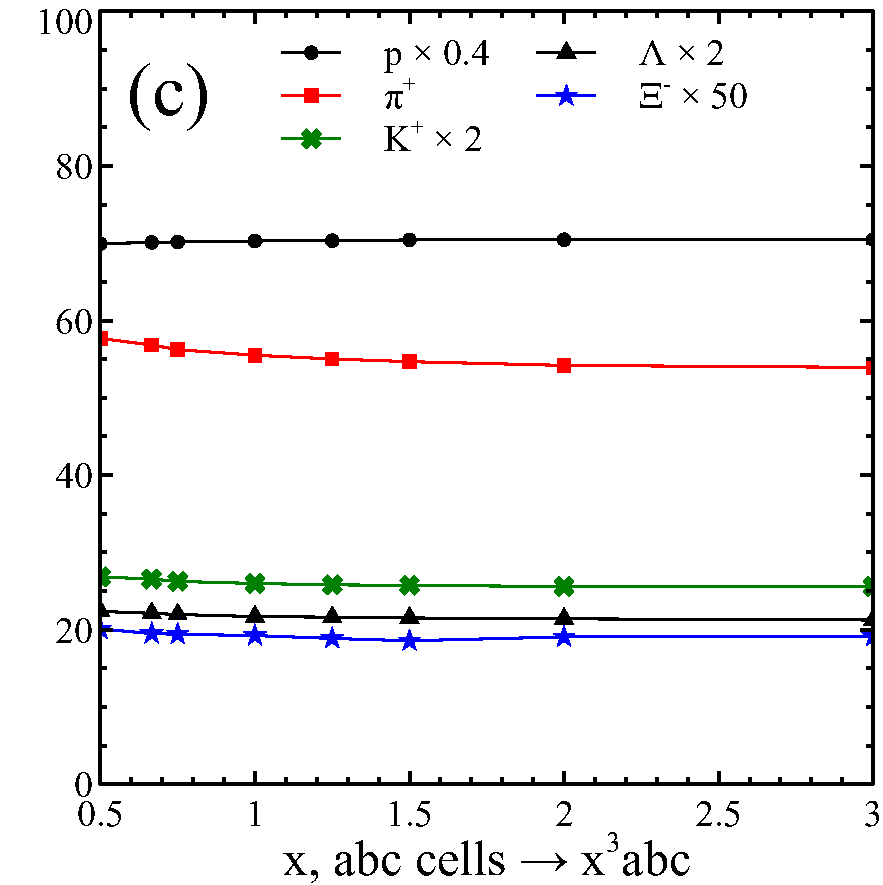
\includegraphics[width=0.49\textwidth]{plots/forced_thermalization/mult_dr.pdf}
  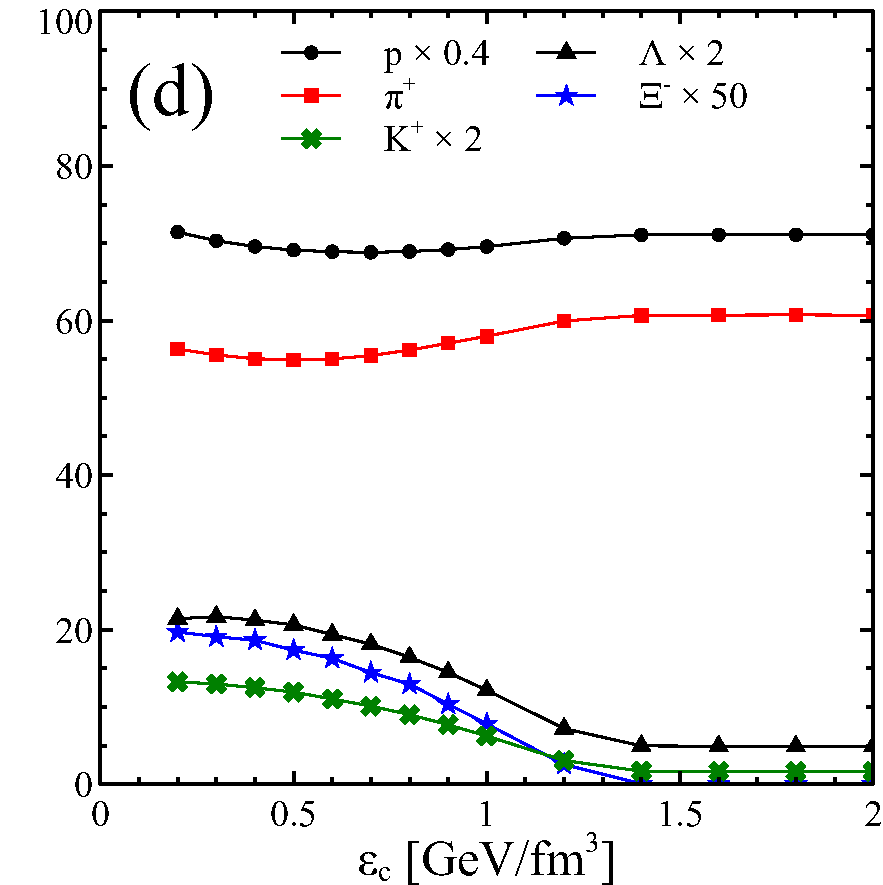
\includegraphics[width=0.49\textwidth]{plots/forced_thermalization/mult_ec.pdf}
  \caption{Central AuAu collision at $\sqrt{s} = 3$ GeV calculated within SMASH
           with effective treatment of N-particle collisions. Final hadron multiplicities
           are shown versus test particle number (a), thermalization period $\Delta
           t_{th}$ (b), grid spacing (panel c, $x$ denotes the factor for number of cells
           in one dimension, $x = 2$ means that the grid is 8 times denser) and energy
           density $\epsilon_c$, above which the thermalization is forced (d).}
  \label{Fig:AuAu_param}
\end{figure}


After studying the effect of forced thermalization in a simple controlled
setup, one can investigate its implications in heavy ion collisions. To understand
our results better, the influence of the thermalization
parameters is also considered, such as the thermalization period $\Delta t_{th}$, the
thermalization grid spacing and the energy density $\epsilon_c$, above which
the thermalization is enforced. In Fig. \ref{Fig:AuAu_param} one can see the
effects of varying these parameters. The ``default'' ones are $N_{test} = 10$, $\Delta
t_{th} = 1$ fm/c, thermalization grid spacing 0.5 fm in the beam direction and 1 fm in
the transverse plane and $\epsilon_c = 0.3$ GeV/fm$^3$. These parameters are varied
one by one, keeping all the rest constant. As one can see in Fig.
\ref{Fig:AuAu_param}, the dependence of the multiplicities on the test
particles number saturate at $N_{test} = 10$, which is the reason this
number was chosen for further investigations. The grid spacing does not affect the
final multiplicities, except a small effect on pions. The grid spacing has no
physical meaning and ideally results do not depend on it. Surprisingly, $\Delta
t_{th}$ also plays a rather small role, even though multiplicities are
decreasing with a larger thermalization period. This is in line with the naive expectation
that larger $\Delta t_{th}$ brings simulation results closer to a pure transport, where
the multiplicity of the strange particles is typically below equilibrium values. The dependency
on $\epsilon_c$ is also predictable - in the limiting case of high $\epsilon_c$,
no thermalization takes place at all, because such high energy densities are
never reached in the collision. So for high $\epsilon_c$ SMASH with forced
thermalization is equivalent to the normal SMASH cascade. This is also
illustrated by Fig. \ref{Fig:AuAu_Vec}. For low $\epsilon_c$, a significant
volume is thermalized during the evolution, which drastically increases strange
particles multiplicities. This can be attributed to the fact that hadronic
interactions do not provide as much strangeness production as a statistical
model would predict. In Fig. \ref{Fig:AuAu_Vec} one can also see that the
lifetime of the high-density region is prolonged due to the forced
thermalization. This is in line with the previously described sphere scenario:
transport with forced thermalization becomes closer to the hydrodynamical
regime. The observable consequence of such behaviour may be larger HBT radii,
compared to pure transport.

\begin{figure}
  \centering
  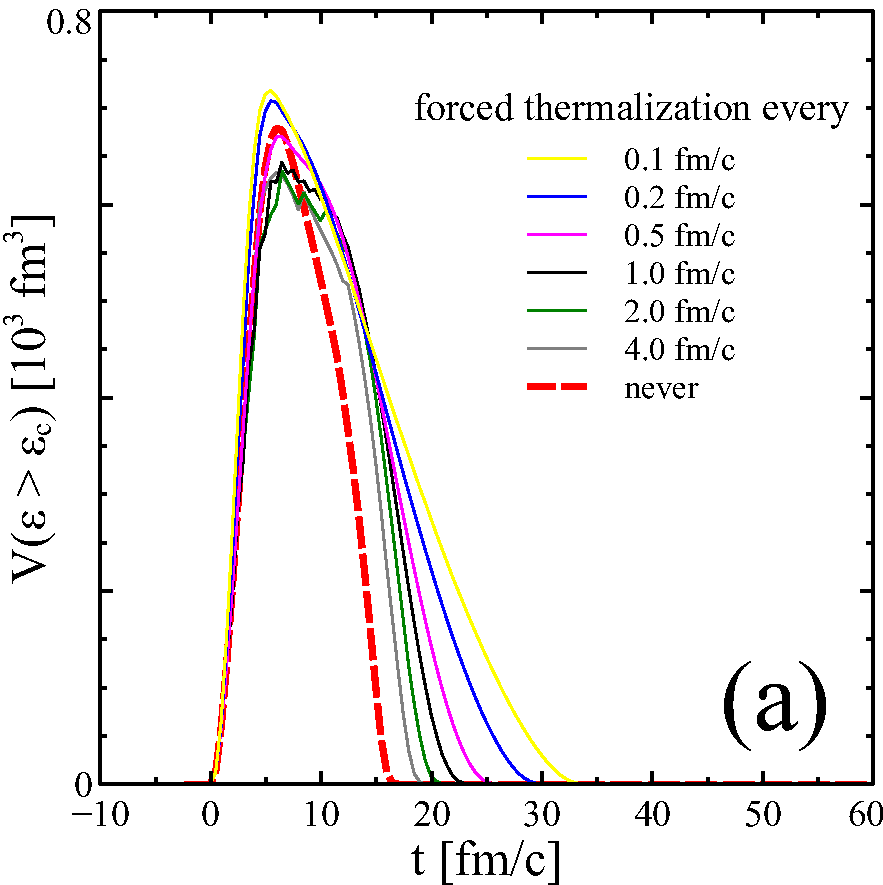
\includegraphics[width=0.49\textwidth]{plots/forced_thermalization/Vec_vs_dt.pdf}
  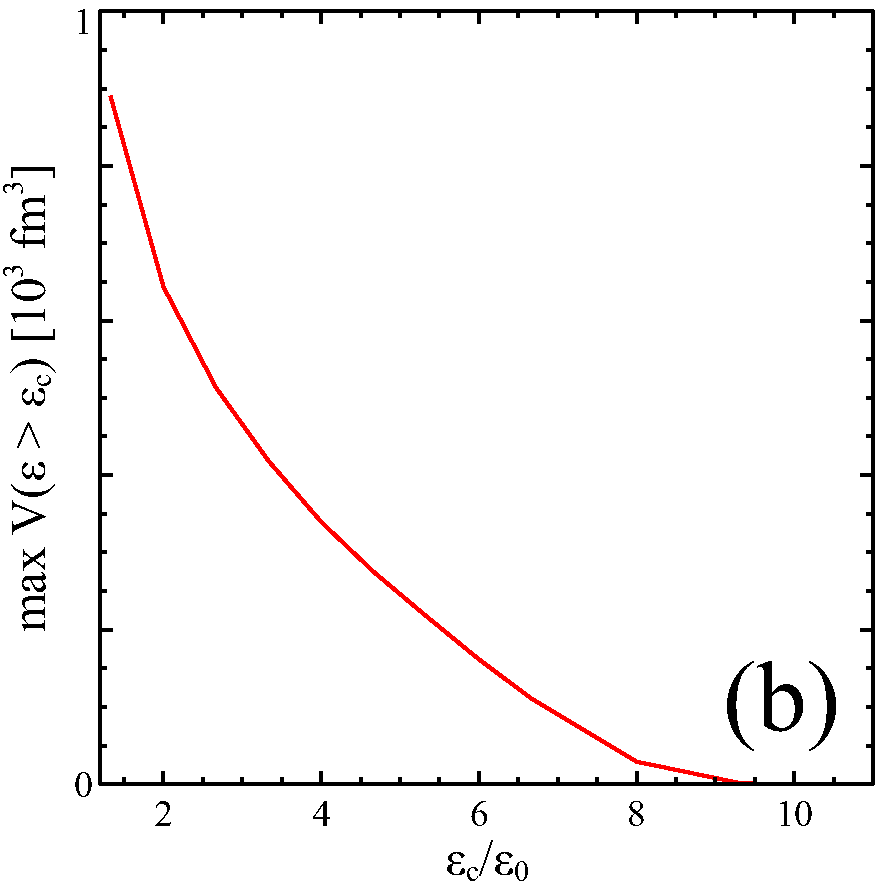
\includegraphics[width=0.49\textwidth]{plots/forced_thermalization/maxV_vs_ec.pdf}
  \caption{Volume of thermalization region versus thermalization period $\Delta
           t_{th}$ (a) and maximal volume versus $\epsilon_c$ (b). Central AuAu collisions
           at $\sqrt{s} = 3$ GeV simulated by SMASH with effective treatment of N-particle
           collisions.}
  \label{Fig:AuAu_Vec}
\end{figure}

Another consequence of our model is a drastic increase of strangeness. This is
not surprising, because in the pure transport strange particles are far from
thermal equilibration. The effects of our forced thermalization on
multiplicities are shown in Fig. \ref{Fig:AuAu_smash_urqmd}, where 3
models are compared: SMASH, SMASH with thermalization, and UrQMD hybrid
\cite{Petersen:2008dd}. The starting time of the thermalization is taken to
match that of the hybrid approach. Energy density $\epsilon_c$ is set to
$2\epsilon_0$, in the UrQMD hybrid particlization energy density is also set to
$2\epsilon_0$. One can see that in terms of multiplicities our model behaves
similarly to the UrQMD hybrid approach, even though the underlying transport
codes have significant differences in terms of resonance properties and
strangeness production. From the Fig. \ref{Fig:AuAu_Tmu} one can see that the
average $T$ and $\mu_B$ inside of thermalization/hydrodynamical region are
similar in all three approaches, which makes comparison sensible.



\begin{figure}
  \centering
  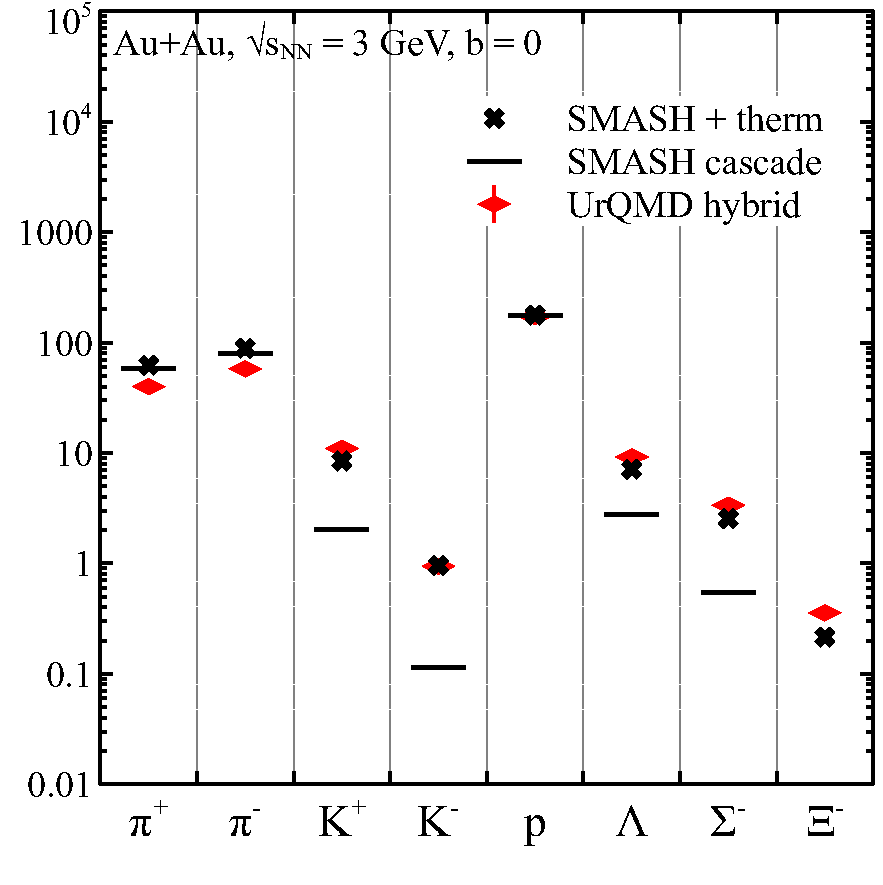
\includegraphics[width=0.5\textwidth]{plots/forced_thermalization/urqmd_smash_compar.pdf}
  \caption{Multiplicities in central AuAu collision at $\sqrt{s} = 3$ GeV
           are compared for SMASH, SMASH with thermalization, and UrQMD hybrid.}
  \label{Fig:AuAu_smash_urqmd}
\end{figure}

\begin{figure}
  \centering
  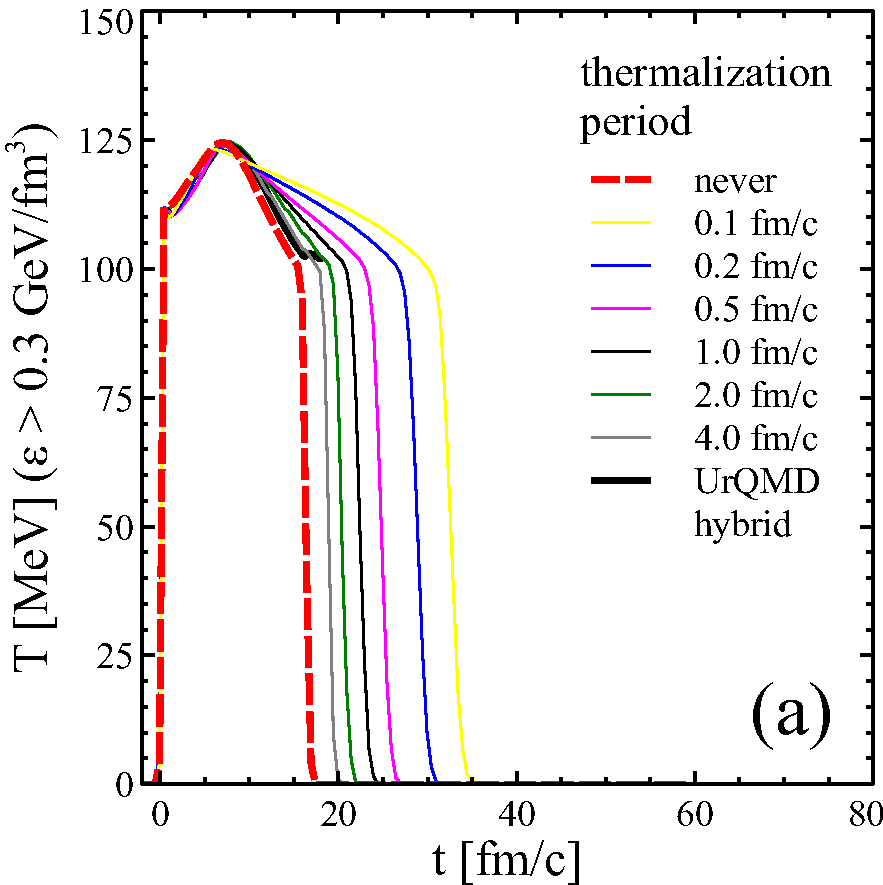
\includegraphics[width=0.49\textwidth]{plots/forced_thermalization/Tav_dt.pdf}
  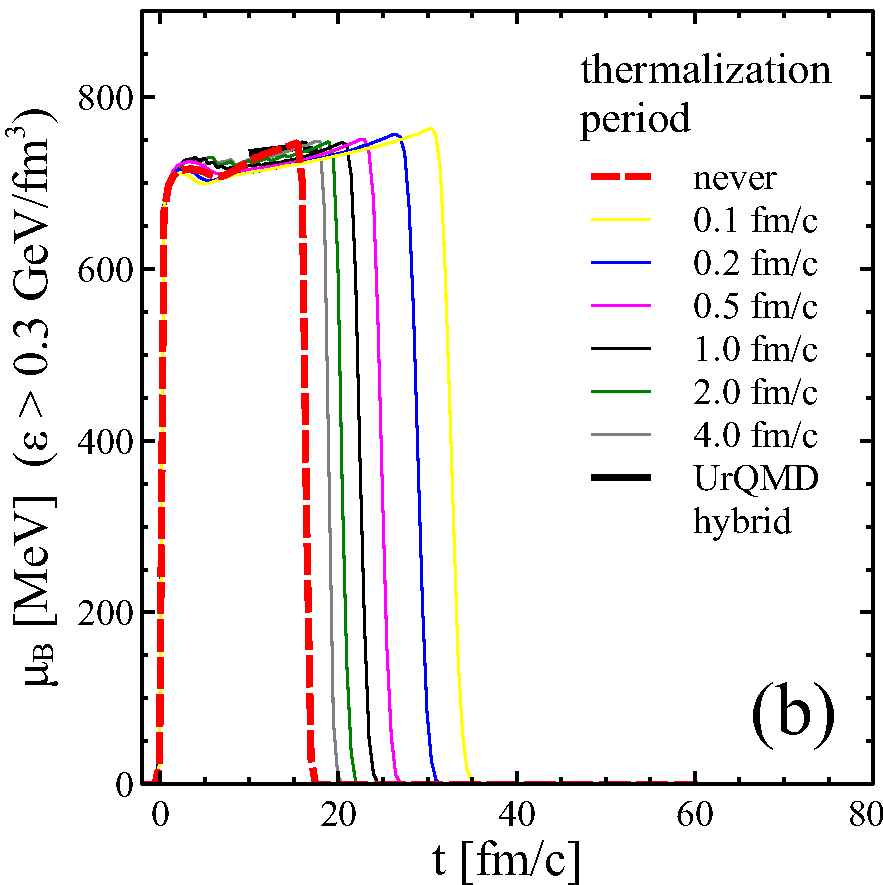
\includegraphics[width=0.49\textwidth]{plots/forced_thermalization/mubav_dt.pdf}
  \caption{Average temperature (a) and baryon chemical potential (b) inside of
           thermalization region for different thermalization periods. Averages are
           weighted with energy density, i.e. $\langle T \rangle = \sum_r T(r) \epsilon(r)
           / \sum_r \epsilon(r)$. Central AuAu collisions at $\sqrt{s} = 3$ GeV simulated
           by SMASH with (solid lines) or without (dashed lines) effective treatment of
           N-particle collisions. Black solid lines correspond to UrQMD hybrid approach.}
  \label{Fig:AuAu_Tmu}
\end{figure}

One more consequence of the forced thermalization is that the pressures in the
longitudinal and transverse directions rapidly equalize. This means that
particles from larger rapidity are redirected to midrapidity and transverse
momentum increases. This is illustrated by Fig. \ref{Fig:AuAu_mean_pt}, which
shows an increase of mean $p_T$ for all particles. One can see that the mean
$p_T$ is insensitive to the thermalization period, but it is quite sensitive to
the forced thermalization itself. The most dramatic effect can be seen for
$K^-$. This is probably because, unlike $K^+$ that can be produced in $NN
\to \Lambda K^+$ reactions, more than 80\% of $K^-$ are produced in the
secondary strangeness exchange $\pi\Sigma\to N K^-$, $\pi\Lambda\to N K^-$ and
$\Sigma^* \to N K^-$. Strangeness exchange reactions preferably deliver their
products to high rapidities. Due to the forced thermalization $K^-$ produced at
high rapidities are redirected to midrapidity.

\begin{figure}
  \centering
  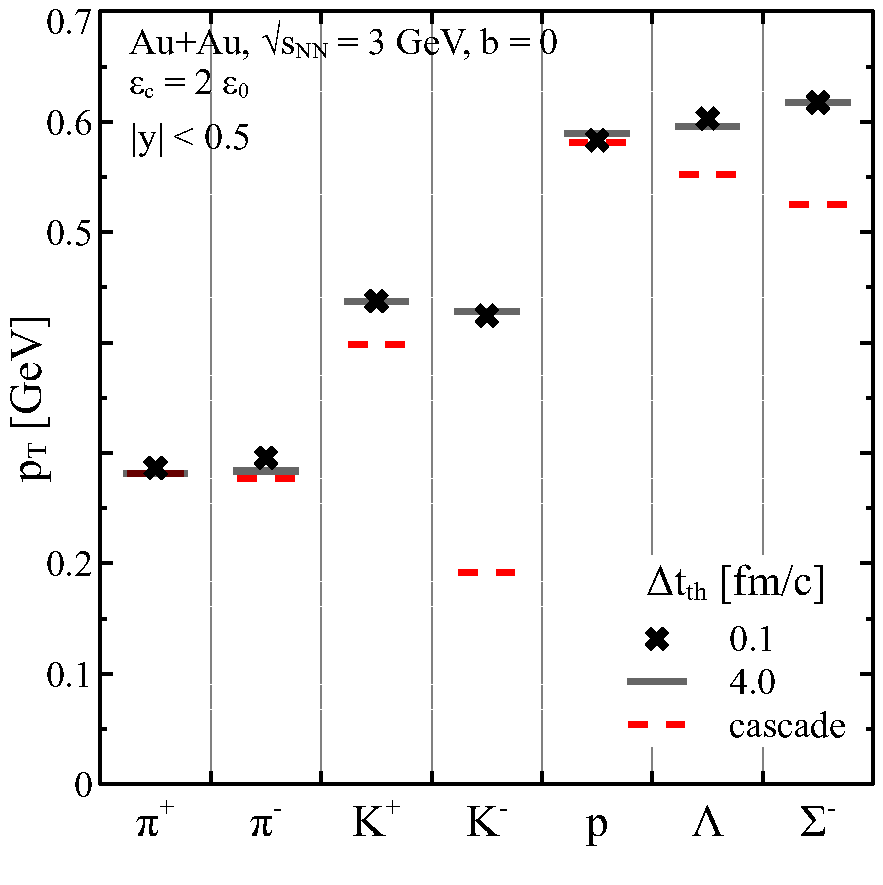
\includegraphics[width=0.5\textwidth]{plots/forced_thermalization/mean_pt.pdf}
  \caption{Mean transverse momentum $p_T = \sqrt{p_x^2 + p_y^2}$ at midrapidity
           in central AuAu collision at $\sqrt{s_{NN}} = 3$ GeV. The model with the forced
           thermalization is compared to cascade.}
  \label{Fig:AuAu_mean_pt}
\end{figure}

\section{Discussion}

A new approach was introduced, where canonical thermalization is performed in a pure
hadronic transport in the regions of high energy density --- the
region, where hydrodynamics would be applied in the hybrid approaches. Unlike
hybrid approaches, this approach automatically guarantees that the high density
and the low density part can exchange particles and that transition
hypersurface is determined dynamically. This approach was implemented and tested
using the SMASH hadronic transport as a basis.

First, several algorithms for sampling particles respecting conservation laws
for all quantum numbers were compared. The Becattini-Ferroni algorithm for
sampling was found to be the most reliable one while its slightly biased version
turned out to be reasonably efficient. In an expanding sphere scenario it was
demonstrated that SMASH with the forced thermalization exhibits intermediate
behaviour between hydrodynamics and transport. The closeness to hydrodynamics
can be regulated by the thermalization frequency - the more often one thermalizes,
the closer the result to hydrodynamics.

Within this novel approach heavy ion collisions were simulated and results were
compared to transport and hybrid approaches. In the forced thermalization approach
more strangeness is produced compared to pure transport, the mean transverse momentum
is increased due to pressure isotropization and the high-density region lives
longer. All these features are qualitatively similar to hybrid approaches.
Note, however, that the problems of hybrid approaches at particlization (discussed
in chapter \ref{chap:cooper_frye}) are absent in the forced thermalization
approach. The dependency of final hadron multiplicities on model parameters was tested
in the forced thermalization approach for Au+Au collisions. Grid spacing did not
influence the multiplicities, the thermalization frequency changed them only slightly.
An interesting behaviour was observed while varying the testparticles number $\Ntest$.
For $\Ntest \geq 10$ multiplicities saturate. For smaller $\Ntest$ one can see a
difference that can be explained by canonical correction. If one increases energy
density $\epsilon_c$ above which thermalization is forced, less particles are
thermalized and therefore less strangeness is produced. Overall, the forced
canonical thermalization approach leads to the expected results and the
straightforward tests look promising.

In the thermalization procedure one needs the EoS to determine local
temperature and chemical potentials. For this purpose a hadron gas EoS was applied,
consistently with SMASH hadron content. One can also apply another EoS,
for example an EoS with a phase transition, but between thermalizations the
propagated degrees of freedom will be still hadrons, which seems inconsistent.
If the quark-gluon plasma only exists at high energy densities and at the edges
of the thermalized blobs the degrees of freedom are still hadronic, this might
allow the direct investigation of EoS of strongly-interacting matter without
explicit hydrodynamic evolution. In the future, these studies can be extended
to higher collision energies and compared to existing experimental data and
can provide predictions for upcoming experiments.